\begin{frame}
\frametitle{}
\begin{center}
{\fontsize{49}{90}\selectfont
{\color{title} Writing Algorithms}}
\end{center}
\begin{itemize}
\item Examples of some simple algorithms
\item Writing a new algorithm
\end{itemize}
\end{frame}

\begin{frame}[fragile]
\frametitle{Feature: Python expressivity - a simple algorithm}
Python is easy to write and read
\begin{block}{Breadth First Search}
\lstinputlisting[firstline=1]{code/bfs.py}
\end{block}
Credit: Matteo Dell'Amico
\end{frame}



\begin{frame}[fragile]
\frametitle{Feature: Python expressivity - a simple algorithm}
Python is easy to write and read
\begin{block}{Erd\H{o}s-R\'enyi Random graph}
\lstinputlisting{code/gnp.py}
\end{block}
\end{frame}

\begin{frame}[fragile]
\frametitle{Feature: Python expressivity - a simple algorithm}
\begin{block}{Erd\H{o}s-R\'enyi Random graph}
\small
\lstinputlisting{code/random_graphs.py}
\end{block}
\end{frame}



\begin{frame}
\frametitle{Degree centrality}
\begin{columns}
\begin{column}{0.5\textwidth}
For a graph with $n$ nodes
\begin{equation*}
C_D(v) = \frac{deg(v)}{n-1}
\end{equation*}
\centerline{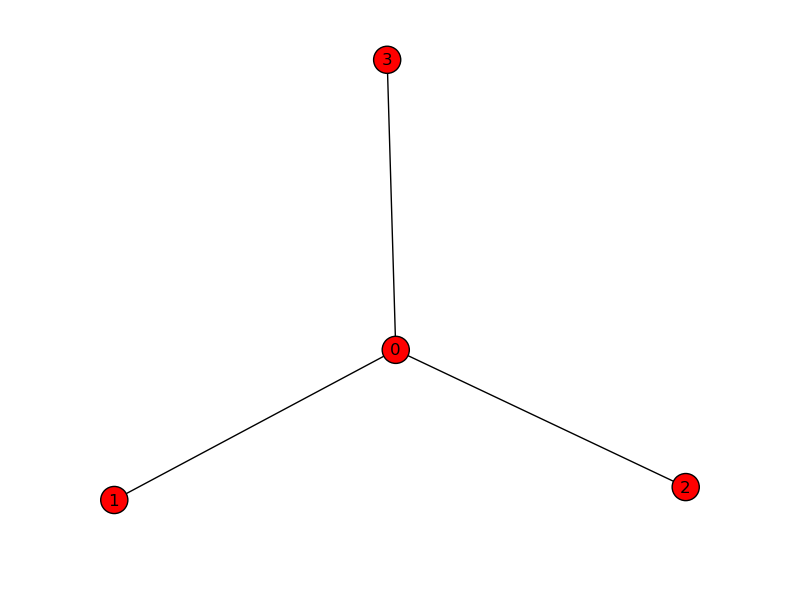
\includegraphics[width=1.0\columnwidth]{star}}
\end{column}
\begin{column}{0.5\textwidth}

\lstinputlisting[firstline=1]{code/degree_centrality.py.doctest}

\end{column}
\end{columns}
\end{frame}



\begin{frame}
\frametitle{Degree centrality 1}
\lstset{showspaces=true,
stringstyle=\color{red}
}
\lstinputlisting{code/degree_centrality1.py}
\end{frame}


\begin{frame}
\frametitle{Degree centrality 2}
\lstinputlisting{code/degree_centrality2.py}
\end{frame}


\begin{frame}
\frametitle{Degree centrality 3}
\lstinputlisting{code/degree_centrality3.py}
\end{frame}


\begin{frame}
\frametitle{Degree centrality 4}
\lstinputlisting[lastline=16]{code/degree_centrality4.py}
\end{frame}


\begin{frame}
\tiny
\frametitle{Degree centrality in NetworkX}
\lstinputlisting{code/nx_degree_centrality.py}
\end{frame}
